\documentclass[11pt, a4j, dvipdfmx]{jarticle}
\usepackage{amsmath}
\usepackage{setspace}
\usepackage{mathtools}
\usepackage[dvipdfmx]{graphicx}  % Include figure files
% \usepackage[varg]{txfonts}
\usepackage{bm}  % bold math
\usepackage{here}
\usepackage{array}
\usepackage[T1]{fontenc}
\usepackage{etoolbox}
\usepackage[top=30truemm,bottom=30truemm,left=25truemm,right=25truemm]{geometry}  % 余白
\usepackage{comment}
\usepackage{cases}
\usepackage[version=3]{mhchem}
\usepackage{layout}
\usepackage{wrapfig}
\usepackage{indentfirst}
\usepackage{txfonts}


%\renewcommand{\indent}{\hspace*{1zw}}
\renewcommand{\abstractname}{}
\renewcommand{\figurename}{Fig.}
\renewcommand{\thefootnote}{\fnsymbol{footnote}}
\renewcommand{\thesection}{\arabic{section}}


\pagestyle{plain}
%%%%%%%%%%%%%%%%%%%%%%%%%%%%%%%%%%%%%%%%%%%%%%%%%%%%%%%%%%%%%%%%%%%%%%%%%%
\makeatletter%% プリアンブルで定義する場合は必須
\patchcmd{\maketitle}{\@fnsymbol}{\@alph}{}{}  % Footnote numbers from symbols to small letters
\long\def\@makecaption#1#2{% \@makecaption を再定義します
  \vskip\abovecaptionskip
  \iftdir\sbox\@tempboxa{#1\hskip1zw#2}%
    \else\sbox\@tempboxa{#1~ #2}  % ここの : を ~ に変更する
  \fi
  \ifdim \wd\@tempboxa >\hsize% 
    \iftdir #1\hskip1zw#2\relax\par
      \else #1~ #2\relax\par\fi  % ここの : を ~ に変更する
  \else
    \global \@minipagefalse
    \hbox to\hsize{\hfil\box\@tempboxa\hfil}  % センタリング
%   \hbox to\hsize{\box\@tempboxa\hfil}%      左詰め
%   \hbox to\hsize{\hfil\box\@tempboxa}%      右詰め
  \fi
  \vskip\belowcaptionskip}
 \DeclareRobustCommand\cite{\unskip
\@ifnextchar[{\@tempswatrue\@citex}{\@tempswafalse\@citex[]}}
 \def\@cite#1#2{$^{[\hbox{\scriptsize{#1\if@tempswa , #2\fi}]}}$}
 \def\@biblabel#1{[#1]}
\makeatother%% プリアンブルで定義する場合は必須

\setlength{\columnsep}{8  truemm}
\setlength{\linewidth}{90 truemm}


\begin{document}


\section{緒言}
\label{sec:introdction}


\subsection{研究背景}
\par
マイクロスイマーとは,水中の微生物に代表される,周辺流体との流体力学的相互作用により,粘性流体中を自己推進する微小な物体の総称である.
マイクロスイマーが分散した流体は,自己泳動しないコロイド粒子が分散した流体とは,大きく性質が異なることが知られている.
マイクロスイマーの挙動の解析は,医療器具などの汚染の原因となるバイオフィルムの形成過程の説明や,
ドラッグデリバリーシステムへの応用など,様々な分野での活用が期待されている.
しかし,流体的相互作用が複雑であり,莫大な計算コストを要することから,解析例が少ない対象でもある.
そのため,マイクロスイマーを解析するには計算負荷を軽減することが重要となる.


\subsection{研究目的}
\par
マイクロスイマー分散系がコロイド分散系と異なる値を示す一例として有効粘度が挙げられる.
有効粘度は,式\eqref{eq:effective_viscosity}のように表される.

    \begin{equation}
        \eta_\mathrm{eff} = \frac{\sigma}{\dot{\gamma}}
        \label{eq:effective_viscosity}
    \end{equation}

\noindent
ここで,$\sigma$は系にかかる応力,$\dot{\gamma}$はせん断速度である.
Rafa\"iらは,泳動するクラミドモナスと泳動しないクラミドモナスとで,
有効粘度の値に違いが見られることを実験により検証しており,
マイクロスイマーの進行方向が異方的であることから,その値の違いが生じると述べられている\cite{}.
そこで,シミュレーション上でマイクロスイマーの進行方向が異方的になる原因と予測される性質を付加し,
その挙動を調べることを本研究の目的とした.
本研究では,マイクロスイマーが,重心が体の中心からずれているbottom heavy性を持ち,
せん断流下に存在することで異方的挙動を再現できると考え,
それらを考慮したシミュレーションを行った.
また,研究の第一歩として,マイクロスイマー単体が存在する系を考えた.

    \begin{figure}[H]
        \centering
        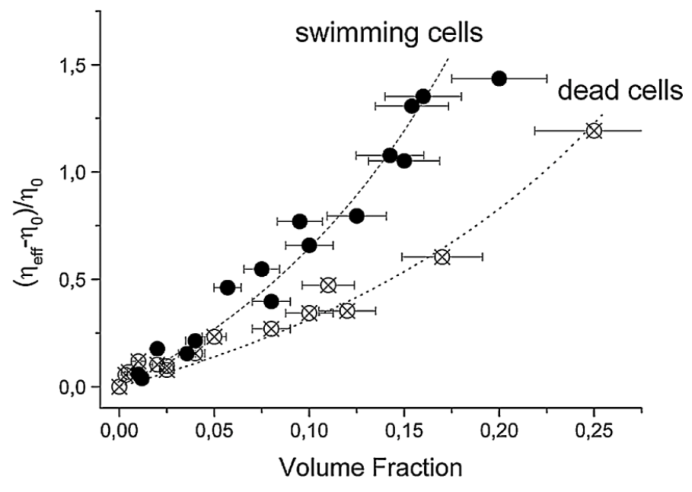
\includegraphics[scale=0.6]{/Users/taiga/Projects/lab/thesis/components/chapter1/figs/previous_research.pdf}
        \caption{泳動の有無による有効粘度の違い}
    \end{figure}

\end{document}
